\section{Appendix 1 }
The following are some characteristics of springs:

Suspension Rate or Stiffness (K) is one of the characteristics that mean that the force needed to compress or extend a suspension spring by a specific amount of distance is known as the spring rate, also known as stiffness. Newtons per millimeter (N/m) are the common units of measurement.

Increased spring rates give the suspension more stiffness, which enhances responsiveness and handling. But too stiff of springs can make for a rough ride. And this will be well discussed in the suspension system conflicts section. \cite{trzesniowski2023suspension}

\section{Appendix 2}
	\begin{itemize}
	
	\item \textbf{Vibration Isolation:} This term means the response of the sprung mass (all components directly supported by the suspension system. Vehicle body and passenger passengers) to the various excitation types from the road. In most cases, \textbf{the transmissibility ratio} (transfer function) is used for evaluating a linear suspension system's vibration isolation ability.
	
	\begin{equation}
		TR=\frac{Z_\text{s}}{Z_\text{0}}
	\end{equation}
	where:
	\begin{itemize}[label=\textbullet]
		\item TR is the transmissibility ratio of the suspension system.
		\item $Z_\text{s}$ is the sprung mass displacement.
		\item $Z_\text{0}$ is the road excitation displacement.
	\end{itemize}
	
	\item \textbf{Suspension Travel (ST):} This means the deflection of the suspension spring or the relative displacement between the sprung mass (Car Body) and unsprung mass (components that are not supported by the suspension system i.e. The wheels and tires).
	\begin{equation}
		ST=\frac{Z_\text{us}-Z_\text{s}}{Z_\text{0}}
	\end{equation}
	where:
	\begin{itemize}[label=\textbullet]
		\item $ST$	is the suspension travel relative to road excitation displacement.
		\item $Z_\text{us}$	is the unsprung mass displacement.
		\item $Z_\text{s}$ is the sprung mass displacement.
	\end{itemize}
	\item \textbf{Roadholding:} The usual force acting between the tire and the road varies as the vehicle system vibrates on the road. The roadholding capabilities, handling, and performance of the vehicle are all influenced by tire vibration, since the cornering force, tractive effort, and braking effort generated by the tire are all associated with the tire's normal load. The displacement of the unsprung mass with respect to the road surface can be used to depict the normal force between the tire and the road during vibration. \textbf{The dynamic tire deflection} is used as a measurable term for evaluating the suspension performance characteristic as this formula:
	\begin{equation}
		DTD=\frac{Z_\text{0}-Z_\text{us}}{Z_\text{0}}
	\end{equation}
	where:
	\begin{itemize}[label=\textbullet]
		\item DTD is the dynamic tire deflection.
		\item $Z_\text{0}$ is the road excitation displacement.
		\item $Z_\text{us}$	is the unsprung mass displacement.
	\end{itemize}
\end{itemize}

\section{Appendix 3}
As an illustration figures \ref{fig:1.1} and \ref{fig:1.2} shows the tradeoffs in suspension design, the response of a passive suspension system at different suspension parameters implemented by suspension mathematical modeling using MATLAB software, it resulted:

A stiffer suspension behavior is required to enhance tire contact with the road-dynamic tire deflection-and the vehicle's dynamic behavior during braking and turning, whereas a softer suspension behavior is required to increase vehicle vibration isolation and enhance passenger comfort. \cite{east2021experimental}

\begin{figure}[H]
\centering
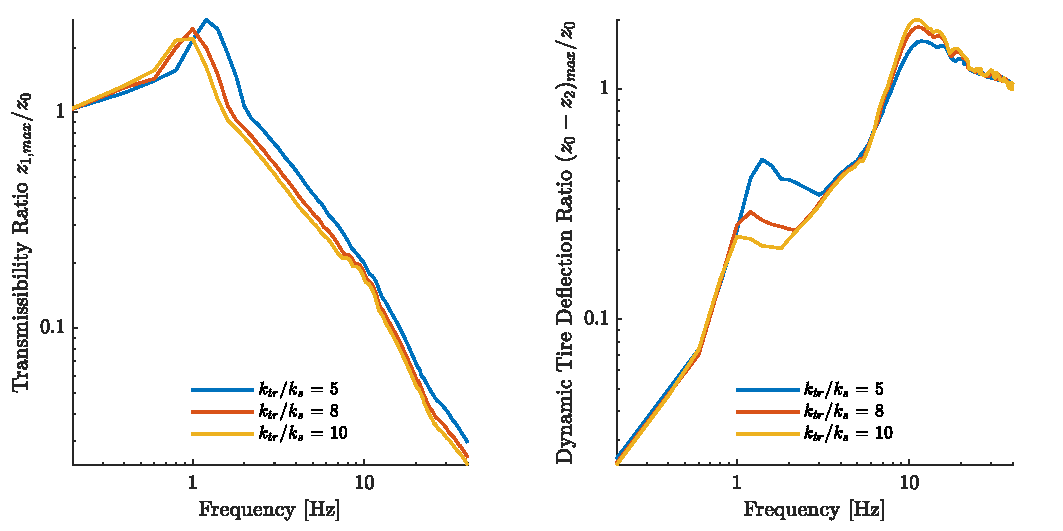
\includegraphics[width=\textwidth]{Stiffness Ratio.pdf}
\caption{Transmissibility ratio (left) and Dynamic Tire Deflection (right) as a function of frequency for the sprung mass of a suspension system with different ratios of tire stiffness to suspension spring stiffness}
\label{fig:1.1}
\end{figure}

\textbf{On the other hand}, As shown in figures 1.3 and 1.4, talking about the damping ratio ($\zeta$), the smaller damping ratio is required to high vibration isolation and good ride quality (lower transmissibility ratio), the natural frequency of the sprung mass or close to the natural frequency of the unsprung mass, to maintain good roadholding capability, higher damping is required. \cite{wong2001theory}

\begin{figure}[H]
\centering
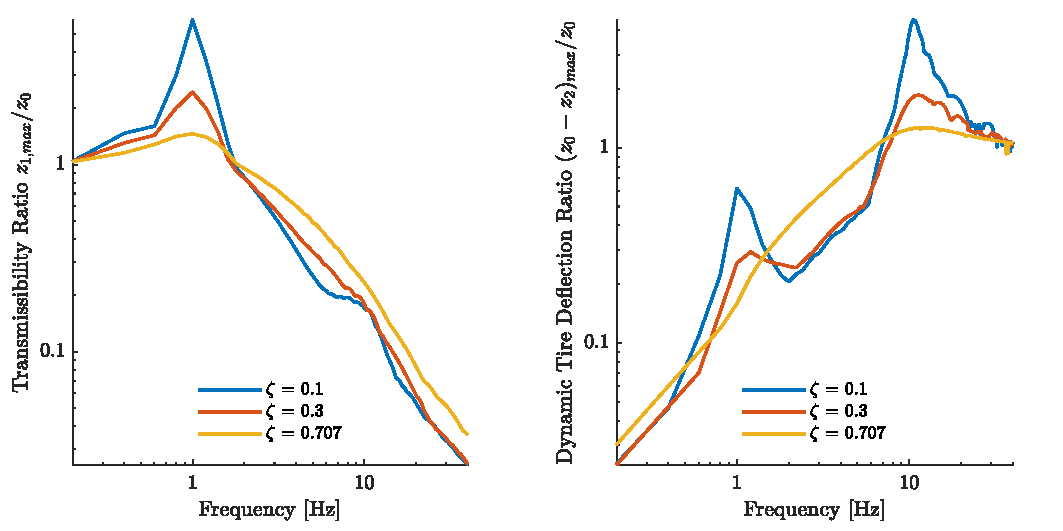
\includegraphics[width=\textwidth]{Damping Ratio.pdf}
\caption{Transmissibility ratio (left) and Dynamic Tire Deflection (right) as a function of frequency for the sprung mass of a suspension system with different damping ratios.}
\label{fig:1.2}
\end{figure}

And this presents a very difficult challenge for the designers, who have to make some compromises to strike a balance barely that is appropriate for maintaining the luxurious and safe driving experience of the vehicle. Furthermore, these compromises affect overall driving experience or vehicle safety and handling. \cite{east2021experimental}

For talking about \textbf{compromises in better overall driving experience} or ride quality, the International Standard IS0 2631 provides an extensive basis for characterizing human tolerance to whole-body vibration. The guide provides three different limits for whole-body vibration: Exposure limit, fatigue, and Reduced comfort. And is suggested for use in industry and in the evaluation of vibratory environments in transport vehicles. And may be considered as guiding for designers in determining the trade-off limits between vehicle road holding and ride comfort reduction. \cite{oborne1983whole}

\textbf{Exposure limits:} which, unless there is a specific reason, should not be exceeded in order to preserve safety (or health).

\textbf{Fatigue or decreased proficiency boundaries:} They pertain to maintaining operational efficiency and are applicable to jobs like operating a tractor or a road vehicle (driving for many hours).

\textbf{Reduced comfort boundaries:} which deal with maintaining comfort in transportation vehicles and are associated with activities like eating, writing, and reading in a car. \cite{east2021experimental}, \cite{oborne1983whole}\\
\textbf{-Road Holding}\\
On the other hand, talking about \textbf{compromises in road holding}, when a vehicle travels on the road, many factors may affect the vehicle holding cause instability. Among the problems related to car instability, reduced road holding in steering or braking or roll over condition, and this is the most dangerous phenomenon. All passengers and goods on board are threatened when the vehicle get instability in the road. Even the life of the car user may not be guaranteed once the instability accident occurs. Developed countries have better road conditions so that cars can travel at very high speeds. But this is not enough to avoid reduced road holding in all driving conditions. \cite{nguyen2023establishing}

In general luxury cars typically have suspension systems that prioritize comfort over handling dynamics, which may cause the car to lose stability when braking and turning at specific high speeds. As a result, these vehicles offer a comfortable ride and are adept at swallowing bumps, but handling and control are compromised. However, the suspension of sports cars is usually designed with a focus on handling, meaning that while improving the road holding and stability, ride quality and comfort are compromised. Therefore, there is a trade-off between comfort and vehicle control when using passive suspension systems (PSS). \cite{kuber2014modelling}